\graphicspath{{chapters/notes/02/images}}
\chapter{Coverage}

\section{Computing coverage}
The three key concepts needed when performing genomics analysis are the local and global coverage and allelic fraction.

    \subsection{Local coverage}
		The local coverage $cov$ at position (base) $i$ is the number of reads that span $p_i$.

    $$cov = \# r_i : r_i \in p_i$$

    \subsection{Allelic fraction}
		The allelic fraction $AF$ at position $i$ is the proportion of reads that supports the reference (or alternative) base in $p_i$ over the total number of reads that span $p_i$.

    $$AF = \frac{\# r_{alternative_i\ (reference_i)}}{\# r_i} : r_i\in p_i$$

    \subsection{NGS global coverage}
    The Lander-Waterman equation is used to compute NGS global coverage.
    The equation is:

    $$C = \frac{L * N}{G}$$

    Where $C$ is the global coverage, $G$ is the haploid human genome length, $L$ the read length and $N$ the number of mapped reads.

\section{Mapping in NGS}
When mapping NGS reads to a reference genome the number of correctly mapped reads is always lower than expected.
This is due to sequencing or aligning errors or due to major translocations that will impair a good mapping of the reads.
When considering which part of the reference genome is covered by the mapped reads, a distinction between physical and sequence coverage has to be made.
A schematic representation of the problem is displayed in figure \ref{fig:seq_phys}.

\begin{figure}[H]
    \centering
    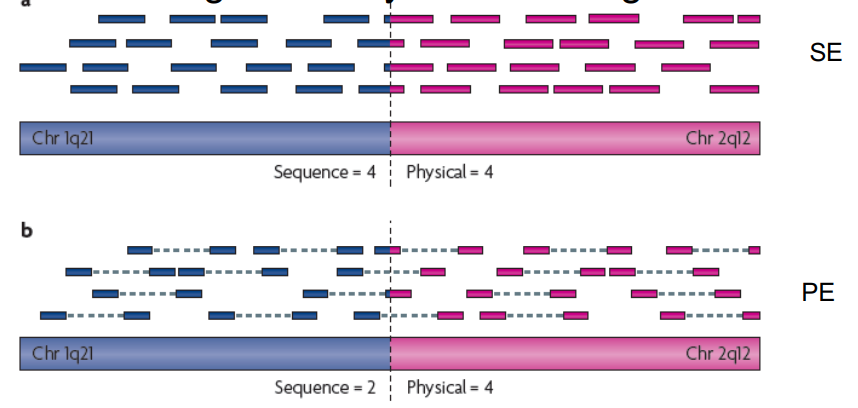
\includegraphics[width=0.5\textwidth]{seq_phys.png}
    \caption{Schematic difference between sequence (on the left) and physical coverage (on the right).}
    \label{fig:seq_phys}
\end{figure}

    \subsection{Sequence coverage}
    Sequence coverage is the amount of oversampling (how many times a base is sequenced).
    It is needed to detect nucleotide alterations with high sensitivity.
    To do so for the 3 billion bases of the human genome a $30$-fold coverage on average ($30X$) is usually required.
    This means that $90$ million of bases need to be mapped for each sample.

    \subsection{Physical coverage}
		The expected distance between the paired reads is used to uniquely place the reads on the genome.
    Physical coverage refers to the average number of times a base is read or spanned by paired end reads.
    Unexpected read pairs are used to detect structural anomalies.
    So, while sequence coverage refers to a single base resolution, physical coverage refers to structural coverage of the genome.

\section{Tuning coverage}
In some experiments setups there's the need to carefully control the amount of intended coverage.

    \subsection{SNP detection}
    SNPs are by definition present in all of the cells of an individual, so only enough redundancy or local coverage to distinguish the reference from the alternative base is needed.
    Ideally for heterozygous SNPs half of the reads will support the reference base while the other half the alternative one.
    Typically to perform this kind of detections only $10$ to $15X$ coverage is needed.

    \subsection{Subclonal events}
    Subclonal events from a tumour or hematopoietic sample are not harboured by all the cells in an individual, so the coverage must be increased with respect to the one needed for SNPs detection.
    The same approach must be taken to detect momozygous mutations and low abundant events, like low-expression transcripts and to reduce the effect of weak binding in chIP-seq.

    \subsection{Amplicon-based approaches}
    Amplicon sequencing is a highly targeted approach that enables researchers to analyse genetic variation in specific genomic regions.
    The ultra-deep sequencing of PCR products or amplicons allows for efficient variant identification and characterization.
    This methods uses oligonucleotide probes designed to target and capture regions of interest, which are amplified by PCR and sequenced by NGS.

        \subsubsection{Heterozygous deletion of PTEN}

        \begin{figure}[H]
            \centering
            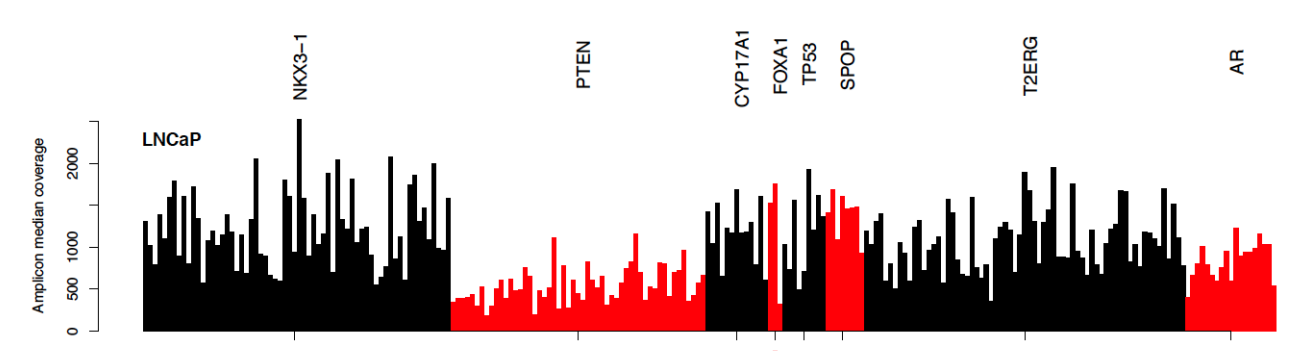
\includegraphics[width=0.5\textwidth]{local_coverage.png}
            \caption{Example of local coverage of $10$ genes for cell line LNCaP. On the x axis genomic location, while on the $y$ axis the amount of amplicons sequenced.}
            \label{fig:local}
        \end{figure}

        In figure \ref{fig:local} a barplot representing the local coverage (y axis) in the gene locations (x axis) can be observed.
        The coverage is on average about $600x$ and it's not evenly distributed, as it typically is for this kind of experiment.
        Averaging the coverage for each gene it is clear how for PTEN it is significantly less.
        Since some coverage is still present for that gene the most probable event to have caused this type of event is an heterozygous deletion.

        \subsubsection{Homozygous deletion of PTEN}

        \begin{figure}[H]
            \centering
            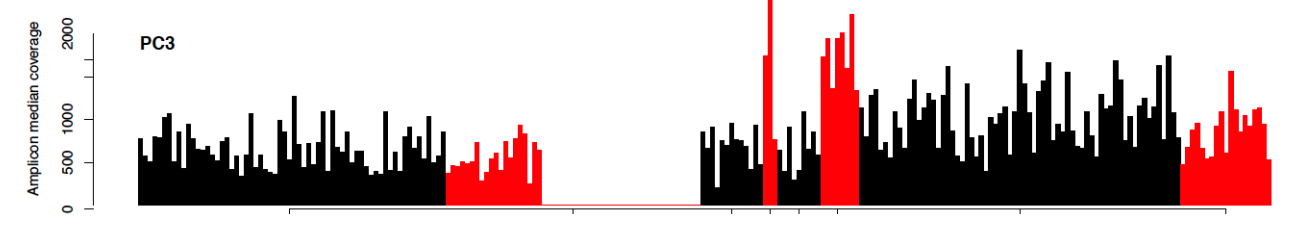
\includegraphics[width=0.5\textwidth]{local_coverage1.png}
            \caption{Example of local coverage of $10$ genes for cell line PC3. On the x axis genomic location, while on the $y$ axis the amount of amplicons sequenced.}
            \label{fig:local1}
        \end{figure}

        In the plot \ref{fig:local1} from a different cell line a clear monoallelic deletion and a partial biallelic deletion of PTEN can be observed.

        \subsubsection{Amplification of AR}
        \begin{figure}[H]
            \centering
            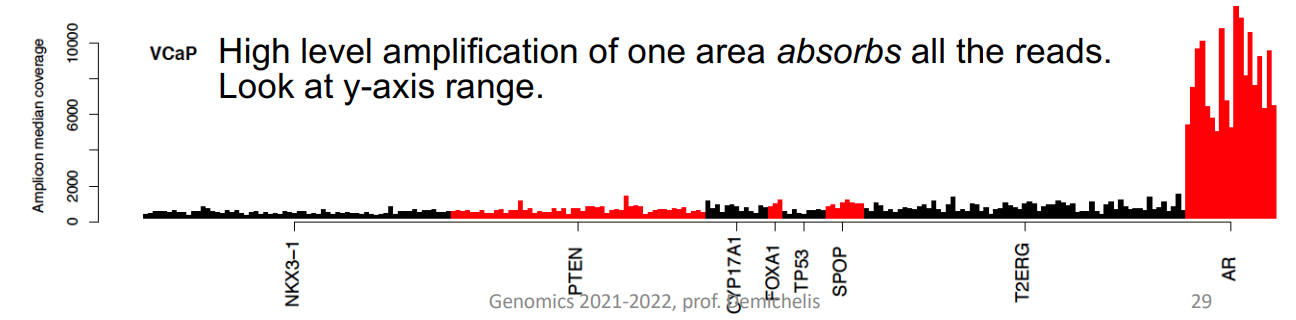
\includegraphics[width=0.5\textwidth]{local_coverage2.png}
            \caption{Example of local coverage of $10$ genes for cell line VCaP. On the x axis genomic location, while on the $y$ axis the amount of amplicons sequenced.}
            \label{fig:local2}
        \end{figure}

        In figure \ref{fig:local2} a massive amplification of the antigen receptor typical of prostate cancer can be seen.
        This massive amplification is probably due to a mistake of the assay.
        Amplification on the AR does not allow for the analysis and discovery of other copy number variations because all of the reads will be mapped to the AR site.

    \subsection{NGS-based approaches}
    NGS-based approach are based on the sequencing of all of the sample genome, skipping the probing and amplification passages.

        \subsubsection{Advantages over amplicon-based approaches}
        With this type of approaches it is easy to increase the experimental coverage at later point in time.
        It is enough to perform another run of sequencing on the same sample or library and then combine the output from different runs to increase coverage.
        This isn't possible with array-based technologies.

        \subsubsection{Problems of NGS-based approaches}
        There are limiting factors to be considered when performing NGS DNA sequencing experiments.
        In particular:

        \begin{multicols}{2}
            \begin{itemize}
                \item Repeated regions are difficult to sequence and map correctly.
                \item Structural information are difficult to obtain.
            \end{itemize}
        \end{multicols}

        This problems could be mitigated by increasing the read length, but this would make the sequencing process more error prone.
        There is a need to make a trade-off between read length and single-base accuracy.

\section{Databases for NGS analysis}
Two very known databases for NGS analysis are:

\begin{multicols}{2}
    \begin{itemize}
        \item Genome Reference Consortium.
        \item USCS Genome Browser.
    \end{itemize}
\end{multicols}

    \subsection{Genome reference consortium}
    The genome reference Consortium assembles a reference genome reflecting the most common sequences in population at each position while tracking information on polymorphisms.

    \subsection{USCS genome browser}
    The USCS Genome Browser allows to  select a reference genome and query all of its known features.
